\documentclass[11pt,a4paper]{article}
\usepackage[top=3cm, bottom=3cm, left=2.5cm, right=2.2cm]{geometry} %geometry of page
\usepackage[hidelinks]{hyperref} %reference links
\usepackage{fancyhdr} %header and footer control
\usepackage{minted} %source code syntax highlighting
\usepackage{qrcode} %qrcode links
\usepackage{graphicx} %images
\usepackage{parskip}

\linespread{1.3}
\emergencystretch 3em

% Set Header and Footer
\fancyhead{}
\fancyhead[L]{\textbf{Lab 3: Servo}}
\fancyhead[R]{max.champneys@sheffield.ac.uk}
\fancyfoot{}
\fancyfoot[L]{\thepage}
\fancyfoot[R]{MAC 233 Arduino Labs, School of MAC, University of Sheffield}

% Create Document
\begin{document}
\pagestyle{fancy}

\section*{Prerequisites}
This worksheet builds upon the theory of how to use an external pin that was covered in the Lab 2 worksheet. Whilst you won't need any code from Lab 2, you will need to have covered how to use a breadboard and how to wire up an external output to an Arduino pin. Out of your Arduino pack, you will need: 1 Arduino, 1 breadboard, 1 servo, and 3 jumper cables.

\section*{Objectives}
The objective of today's lab is to learn how to control a servo using the inbuilt Arduino Servo Library: \url{https://docs.arduino.cc/libraries/servo/}.

This worksheet will take you through the steps of how to connect an external servo to your Arduino and create a sketch that rotates the servo in increments of 30 degrees. Once the sketch reaches 180 degrees (the maximum rotation of most servos), the sketch will reset the servo to zero degrees and start incrementing in steps of 30 degrees again.

\section*{Understanding how a servo works}
Within the remit of this lab, a servo (or servomotor) is a physical device used to control rotary motion. On an Arduino, servos (and some other analogue devices) need to be controlled using Pulse Width Modulation (PWM). You have covered the theory of PWM during your electronics lectures; therefore, this lab will not go into detail about PWM (for more details see: \url{https://docs.arduino.cc/learn/microcontrollers/analog-output/}).

It is important to understand that depending on the Arduino you are using, not every pin can be used for PWM output. On the Arduino Nano Every, the digital pins that can handle a PWM output are pins: 3, 5, 6, 9, 10 (marked with a \verb|~| on the Nano Every pinout diagram: \url{https://docs.arduino.cc/resources/pinouts/ABX00028-full-pinout.pdf}).\footnote{Strictly speaking, the Servo library does not use those pins' hardware PWM at all: it times the pulses itself using an interrupt, so any digital pin would work. Throughout this lab we treat the Servo library as though it were ordinary PWM, which it is for our purposes.}

On an Arduino there is an inbuilt Servo library that abstracts the PWM complexities and helps us control a servo (or an Electronic Speed Controller connected to a DC motor). Using this library, we can simply write the desired position of the servo directly. The number of degrees of rotation available on most servos is: 0\textrightarrow 180.

A servo has three wires coming out of it: a \textit{power} cable, a \textit{ground} cable, and a \textit{signal} cable. The power cable is usually red, the ground cable is usually black or brown, and the signal cable is usually white or orange. As you might be able to guess, power and ground will take +5V (other servos might need different voltages) and 0V respectively and provide power to the servo, while the signal wire expects our PWM signal.

\section{Creating the circuit}
The circuit needed for this worksheet uses one jumper cable for each of the servo's three wires:
\begin{itemize}
    \item Arduino Pin D9 \textrightarrow{} servo signal cable,
    \item Arduino +5V \textrightarrow{} servo power cable,
    \item Arduino GND \textrightarrow{} servo ground cable.
\end{itemize}
Use the pinout diagram linked above to find each of these pins on your Arduino.

\section{Set up the Servo library}
The first thing we need to do is create a blank sketch. To do this, open Arduino IDE and go to `File'\textrightarrow `Examples'\textrightarrow `01.Basics'\textrightarrow `BareMinimum'. Once this has opened, we can set up the Servo library.

In the global scope (the top of the file), enter the code below. This code links our sketch to the Servo library, defines a new named pin called \verb|SERVO_PIN| on pin D9, and then creates an instance of the Servo library called \verb|servo| for us to interact with.
% not pulled from the sketch: these three lines sit apart in the sketch, with
% explanatory comment blocks between them that would swamp this step
\begin{minted}{arduino}
#include <Servo.h>
#define SERVO_PIN 9
Servo servo;
\end{minted}

Next, we declare the array (vector) of integer values we want the sketch to output. For now, this will be every 30 degrees from 0 to 180. Put the code below into the global scope, underneath the previous code. This works in the same way as Lab 1 and Lab 2; however, instead of an array of dots and dashes, we now have an array of degrees to rotate the servo to.
\inputminted[
    autogobble, stripnl,
    rangestartstring={int output[7]},
    rangestopstring={int output_position = 0;},
]{arduino}{../lab-3-servo.ino}

\section{Setup function}
The setup function needs to do four things: 1 - start the serial connection for debugging, 2 - set the position in the output, 3 - set the output pin and attach it to the Servo library, 4 - pause, then report that the system is ready. The code in the following sections goes into the `setup' function, in the order shown.

\subsection{Set up debugging}
The first thing to do in any sketch is to start the serial connection. This allows us to monitor what the Arduino is doing, by displaying messages in the serial monitor at certain points throughout the sketch.

\inputminted[
    autogobble, stripnl,
    rangestartstring={Serial.begin(9600);},
    rangestopstring={Serial.begin(9600);},
]{arduino}{../lab-3-servo.ino}

\subsection{Set up output}
In the global scope, we have already declared the desired output; however, it is always good practice to reset any variables that could be changed at different points during the sketch. In our case, this is simply the current position in the degree output.

\inputminted[
    autogobble, stripnl,
    rangestartafterstring={// reset the position},
    rangestopbeforestring={// set the servo pin to output},
]{arduino}{../lab-3-servo.ino}

\subsection{Set up the servo}
In the global scope, we have created the servo, but we now need to tell the Servo library which pin it is connected to. In our case this is pin D9, which we previously named \verb|SERVO_PIN|. First, we set pin D9 to be an output pin. We can then attach pin D9 to the Servo library. Finally, we can set the servo to 0 degrees.

\inputminted[
    autogobble, stripnl,
    rangestartafterstring={// set the servo pin to output},
    rangestopstring={servo.write(0);},
]{arduino}{../lab-3-servo.ino}

\subsection{System ready}
The last thing to do in the `setup' function is to pause the system for 3 seconds, and then display the message `System Ready' in the serial monitor.

\inputminted[
    autogobble, stripnl,
    rangestartafterstring={// pause the system},
    rangestopstring={Serial.println("System Ready");},
]{arduino}{../lab-3-servo.ino}

\section{Loop function}
Now that we have the setup function sorted, we can concentrate on the loop function. Within the loop function, there are three major steps: 1 - write the correct value to the servo, 2 - determine the next position in the \verb|output| array, 3 - wait two seconds before the next iteration. The code in the following sections goes into the `loop' function.

\subsection{Output to servo}
The top of the `loop' function writes the current value from the output array to the servo. Thankfully, this is one line of code: we look up the current position within the output array, and then tell the servo to move to that value. We also add a second line that displays the same value in the serial monitor, so that we can monitor the progress of the sketch.

\inputminted[
    autogobble, stripnl,
    rangestartafterstring={// move the servo to the correct position},
    rangestopstring={Serial.println(output[output_position]);},
]{arduino}{../lab-3-servo.ino}

\subsection{Determine next position}
Next, the `loop' function determines the next position within the output array. Thankfully, this is the same logic that is used to determine the next position within the dots and dashes array in Lab 1: once we reach the last position in the array, we go back to the start.

\inputminted[
    autogobble, stripnl,
    rangestartafterstring={// determine next position},
    rangestopbeforestring={// wait 2 seconds},
]{arduino}{../lab-3-servo.ino}

\subsection{Wait}
The final step in the `loop' function is to wait two seconds until the next iteration. This is done by telling the Arduino to wait 2000 milliseconds.

\inputminted[
    autogobble, stripnl,
    rangestartstring={delay(2000);},
    rangestopstring={delay(2000);},
]{arduino}{../lab-3-servo.ino}

\section{Try it out on your Arduino}
You now should be able to compile your sketch (`Sketch'\textrightarrow `Verify/Compile') and then upload to your Arduino (`Sketch'\textrightarrow `Upload'). You should see that your Arduino now rotates your servo 30 degrees every 2 seconds until it gets to 180, at which point it restarts back from 0. If you open the serial monitor (`Tools'\textrightarrow `Serial Monitor'), you will also see each angle displayed as the servo moves to it.

\section{Extension}
Once you have a working sketch from the above code, extend the sketch to rotate in 30 degree increments from 0 to 180, and then rotate in 30 degree decrements from 180 back down to 0, without repeating the same degree value twice in a row.

If you finish the above, see if you can combine the servo with an LED (connected to another pin) to flash at given servo positions.

\pagebreak
\section*{Help}
If you are having issues compiling the project or don't understand where each section goes, you can see a complete version of the sketch with additional source code comments at \url{https://github.com/MDCHAMP/MAC233/blob/main/labs/lab-3-servo/lab-3-servo.ino}.

\vspace{2em}

\begin{center}
    \qrcode[hyperlink, height=4cm]{https://github.com/MDCHAMP/MAC233/blob/main/labs/lab-3-servo/lab-3-servo.ino}
\end{center}

\vspace{2em}

Additionally, if you are wondering how the components connect together, the circuit diagram for this lab is below.

\begin{center}
    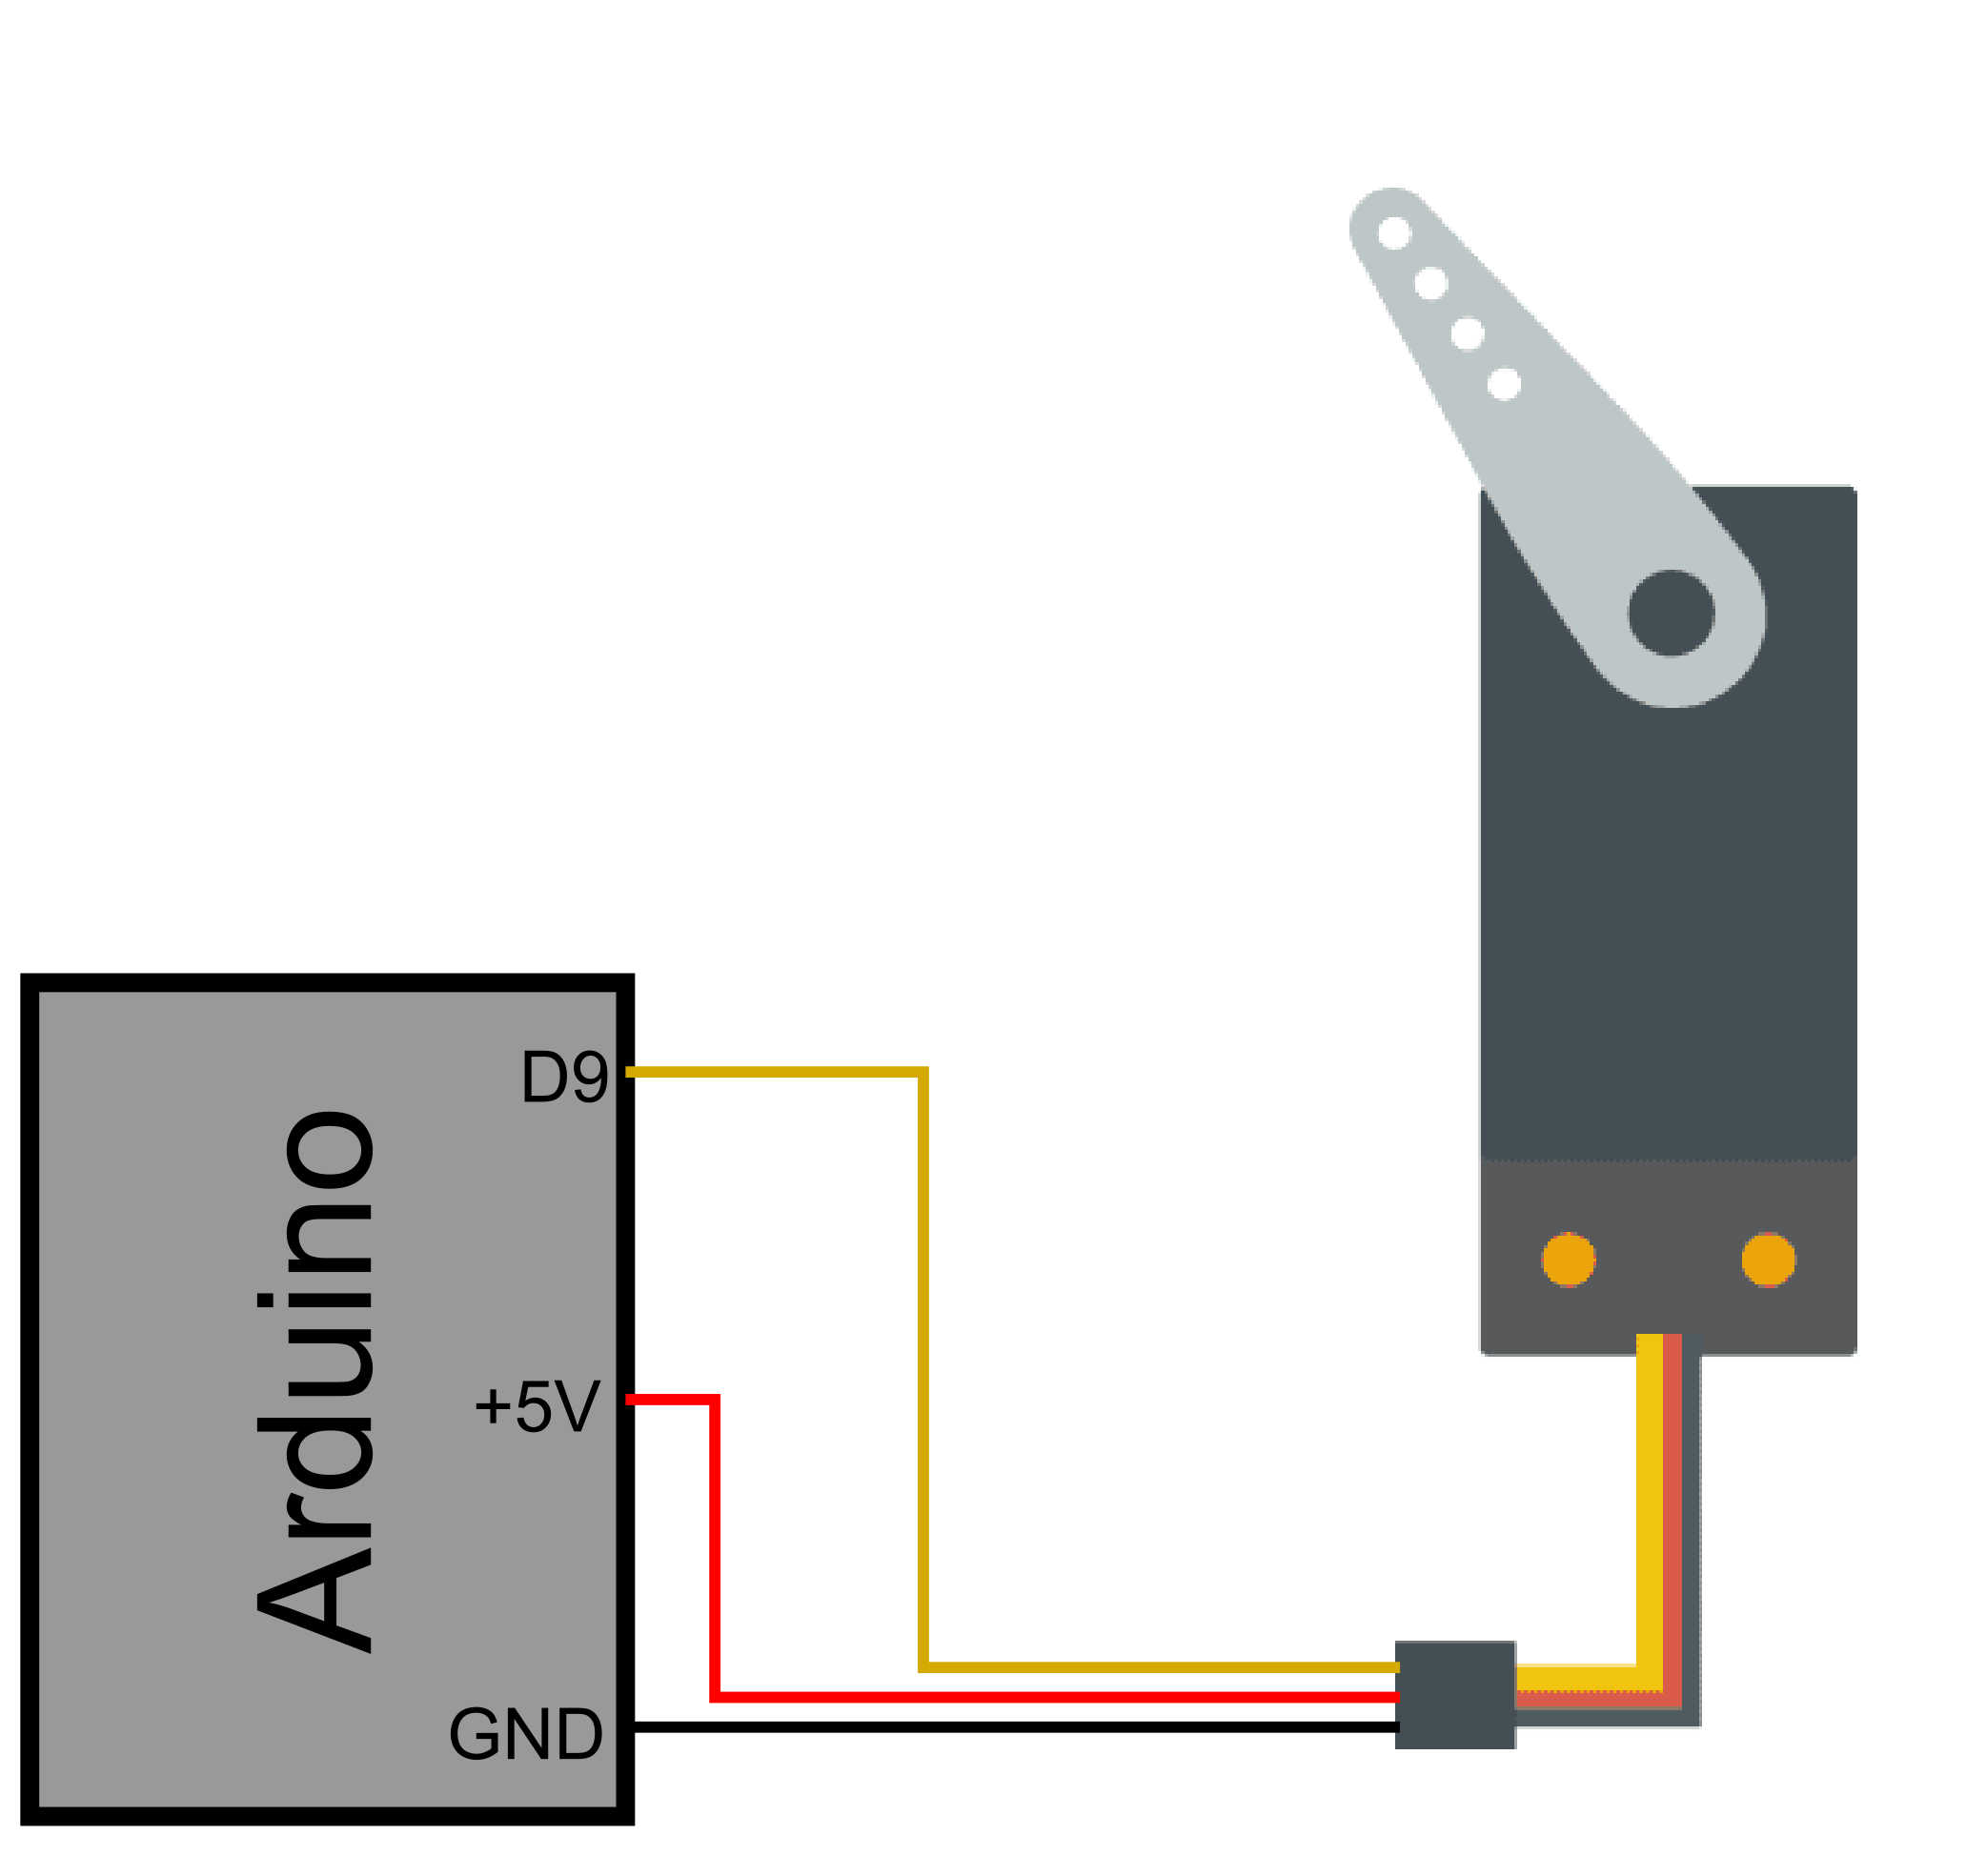
\includegraphics[width=.5\textwidth]{../images/wiring-diagram.png}
\end{center}

\end{document}
